% !TEX program = xelatex
%%%%%%%%%%%%%%%%%%%%%%%%%%%%%%%%%%%%%%%%%
% Beamer Presentation
% LaTeX Template
% Version 1.0 (10/11/12)
%
% This template has been downloaded from:
% http://www.LaTeXTemplates.com
%
% License:
% CC BY-NC-SA 3.0 (http://creativecommons.org/licenses/by-nc-sa/3.0/)
%
%%%%%%%%%%%%%%%%%%%%%%%%%%%%%%%%%%%%%%%%%

\documentclass{beamer}
\usepackage{tikz,lmodern,textpos,hyperref,graphicx,booktabs,appendixnumberbeamer,nth}
\usepackage[export]{adjustbox}
 \usepackage[en-US]{datetime2}

\beamertemplatenavigationsymbolsempty

\mode<presentation>{
  \usetheme{metropolis}
  \setbeamercolor{institute in head/foot}{fg=stanfordRedText}
  \setbeamercolor*{palette tertiary}{use=structure,fg=white,bg=stanfordRed}
}

\title{Examining Crowd Work and Gig Work Through The Historical Lens of Piecework}

\author{\textbf{Ali Alkhatib}, Margaret Levi, Michael Bernstein\\
\texttt{ \href{mailto:ali.alkhatib@cs.stanford.edu}{ali.alkhatib@cs.stanford.edu} ||
         \href{http://twitter.com/_alialkhatib}{@\_alialkhatib} }}

\institute[Stanford]{Stanford University}
\date{\today}

\begin{document}

\begin{frame}
\titlepage
\end{frame}

\begin{frame}{A New Form of Work: On--Demand Labor}
  \begin{itemize}[<+- | alert@+>]
    \item Crowdsourcing
    \begin{figure}
    
\includegraphics[scale=0.3]{figures/amt.png}
    
\includegraphics[scale=0.1]{figures/upwork.png}
    \end{figure}
    \item Gig work
    \begin{figure}
    
\includegraphics[scale=0.1]{figures/uber.png}~~~~~
    
\includegraphics[scale=0.15]{figures/handy.png}
    \end{figure}
  \end{itemize}
\end{frame}


\begin{frame}{Growing Number of Questions}
\begin{itemize}[<+- | alert@+>]
  \item What are the complexity limits of on--demand work?
  \item How far can work be decomposed into smaller microtasks?
  \item What will work and the place of work look like for workers?
\end{itemize}


\end{frame}


\section{Piecework as a lens to understand on--demand work}


\begin{frame}{A (\textit{quick}) Primer on Piecework}
  \begin{itemize}[<+- | alert@+>]
    \item Payment made for \textit{output}, rather than for \textit{time}
  \end{itemize}
\end{frame}


\begin{frame}{An Example: Pieceworkers at the turn of the \nth{20} century}
  \begin{figure}
    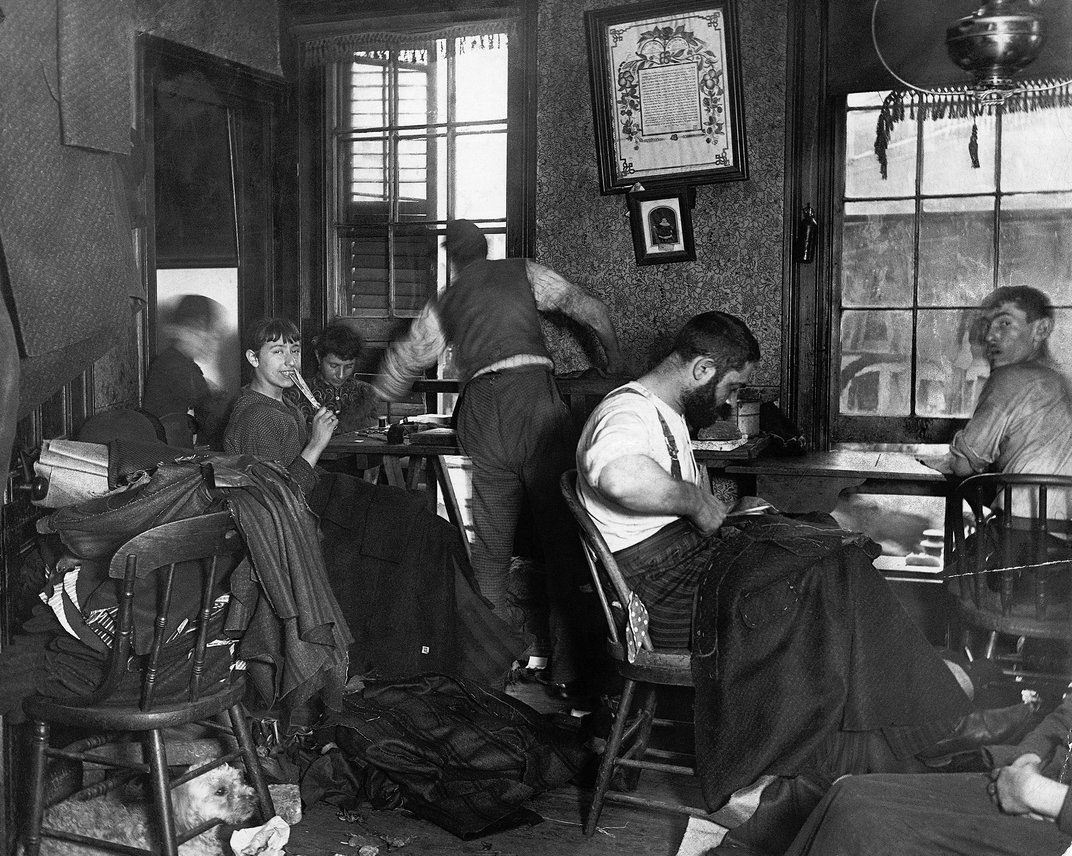
\includegraphics[scale=0.27]{figures/pieceworkers.jpg}  
  \end{figure}
\end{frame}


\begin{frame}{One Question: The Limits on Task Decomposition}
  \begin{itemize}[<+- | alert@+>]
  \item Piecework: Lack of instrumentation limited task decomposition
  \item Today? Tools and technology can track every move workers make
  \item We've hit upon what seems to be an atomic limit on decomposition ---
        cognitive switching between tasks is becoming the main barrier
  \end{itemize}
\end{frame}


\begin{frame}{Future Directions}
  \begin{itemize}[<+- | alert@+>]
  \item If on--demand labor follows the same trajectory as piecework, what can we expect?
  \item If we can design the entire platforms of labor in ways we couldn't imagine a century ago, what can we do to affect different outcomes?
  \end{itemize}
\end{frame}


\begin{frame}
  \frametitle{Contact}
    name: \href{https://ali-alkhatib.com}{Ali Alkhatib} \\
    email: \href{mailto:ali.alkhatib@cs.stanford.edu}{ali.alkhatib@cs.stanford.edu} \\
    twitter: \href{https://twitter.com/_alialkhatib}{@\_alialkhatib} \\
\end{frame}

\end{document} 